% =====================================================================
%  c03 —— PDF p.26–33（原书 p.20–27）
%  §2 二次微分的理论；§2.1 二次微分决定的叶状结构；§2.2 二次微分形式与带状图
% =====================================================================

% ===== 原书 p.20 =====
% §2（原书印「§2. QUADRATIC DIFFERENTIAL の理論」）
\section{二次微分的理论}
% §2.1（原书印「§2.1 QUADRATIC DIFFERENTIAL の定める FOLIATION」）
\subsection{二次微分决定的叶状结构}

本章说明 Strebel 的紧 Riemann 面（或者在它上面给定相异$n$点）上的二次微分理论。
参考书为[St]。这一理论不得不使用单变量函数论中的解析手法，正因如此才可以应用于模空间的胞腔分解。
二次微分的存在性，其理论根据在于从正规族中取出收敛的函数列。

设$X$为紧 Riemann 面，$p_1,\dots,p_n$为$X$上相异点，$D$为由$p_1+\dots+p_n$定义的除子。
$(X,p_1,\dots,p_n)$的二次微分$\omega$，指$(\Omega^1(D))^{\otimes2}$的整体截面。
以下在各点$p_i$处取其单值化参数（uniformizing parameter）$z_i$时，$\omega$可写成
\[
\omega=(a_{-2}z_i^{-2}+a_{-1}z_i^{-1}+\cdots)dz_i^{\otimes2},
\]
此时假定$a_{-2}\neq0$。这时在$X-\{p_1,\dots,p_n\}-(\omega)_0$（此处$(\omega)_0$为$\omega$的零点）上
有两种叶状结构（foliation）$F_r$、$F_i$，定义如下。

取$x\in X-\{p_1,\dots,p_n\}-(\omega)_0$的充分小邻域$U$及其上的单值化参数$z$，则$\omega$可写成
\[
\omega=f(z)dz^{\otimes2},\qquad f(z)=(a_0+a_1z+\cdots)dz^{\otimes2},
\]
其中$a_0\neq0$。于是除$\pm$号外存在唯一的$g(z)$，使$g(z)^2=f(z)$。
令$\psi(z)=\int_x^zg(z)$，则$\omega=\psi(z)$仍是$x$处的单值化参数。（必要时换用充分小的$U$。）
$U$上的曲线族$F_r|_U$，定义为由$T_{r,a}=\{z\mid\psi(z)\in a+i\R\}$（$a\in\R$）给出的族。
因$\psi(z)$除$\pm$号外唯一确定，$F_r|_U$在$X-\{p_1,\dots,p_n\}-(\omega)_0$上决定叶状结构。
同样，$F_i|_U$定义为由$T_{i,b}=\{z\mid\psi(z)\in\R+bi\}$（$b\in\R$）确定的曲线族，
再同样定义整体的$F_i$。又$\psi(z)\colon U\xrightarrow{\ \sim\ }D\subset\C$诱导$\C$的平坦度量，
故$U$上有平坦度量。而$\psi(z)$由$\omega$除$\pm1$外唯一确定，且积分起点的更换只引起平移，
因此在$X-\{p_1,\dots,p_n\}-(\omega)_0$上诱导平坦度量。称之为由$\omega$决定的平坦度量。
对$X$的子集$U$，用$\omega$决定的度量量出的面积记作$\|\omega\|_U$。

\transnote{原文此处把$f(z)$写成$(a_0+a_1z+\cdots)dz^{\otimes2}$，即$dz^{\otimes2}$重出了一次；
下一句又把$\psi(z)$误印作$\omega$。两句均照原文排印。}

下面看$F_r$在$p_1,\dots,p_n$以及$(\omega)_0$处的样子。

（1）$p_1,\dots,p_n$处的样子。设$p_i$处的局部参数为$z$，则$\omega=(a_{-2}z^{-2}+$
% ===== 原书 p.21 =====
$a_{-1}z^{-1}+\cdots)dz^{\otimes2}$，且$a_{-2}\neq0$，故存在某个$g(z)$，
使$g(z)=(b_{-1}z^{-1}+b_0+\cdots)$，其中$b_{-1}\neq0$。
取$p_i$的充分小邻域$U$以及$U-\{p_i\}\ni p_0$，令$\psi(z)=\int_{p_0}^zg(z)dz$。
$w=\psi(z)$是多值函数，记其反函数为$\tau$，则$\tau$是周期为
$\oint g(z)dz=2\pi i\cdot b_{-1}$的周期函数。
\[
\begin{array}{ccc}
\C\supset(\operatorname{Im}\psi) & \xrightarrow{\ \tau\ } & U-\{p_0\}\\[2pt]
\downarrow & & \downarrow\\[2pt]
w & \mapsto & \tau(w)
\end{array}
\]

现引入新变量$t=\exp\left(\frac{w}{b_{-1}}\right)$，则$t$是$U$上$p_i$周围的单值化参数。
属于$F_r$的曲线族由$w=b_{-1}\log(t)\in a+i\R$给出。此时
\[
t=\exp\left(\frac{a+i\theta}{b_{-1}}\right)=\exp\left(\frac{a}{b_{-1}}\right)\exp\left(\frac{i\theta}{b_{-1}}\right)
\qquad(\theta\in\R)
\]
是该曲线的参数表示，其图形按下列情形区分。

\begin{enumerate}[label=(\arabic*),leftmargin=2.6em,itemsep=2pt,topsep=4pt]
\item $b_{-1}\in\R$的情形。$T_a$是与绕$p_i$一周的$S^1$同胚的曲线，长度为$2\pi b_{-1}$。
\item $b_{-1}\in i\R$的情形。$T_a$同胚于连结$p_i$与另一点的半直线。
\item $b_{-1}\in\C-\R-i\R$。$T_a$呈涡旋状。
\end{enumerate}

\begin{center}
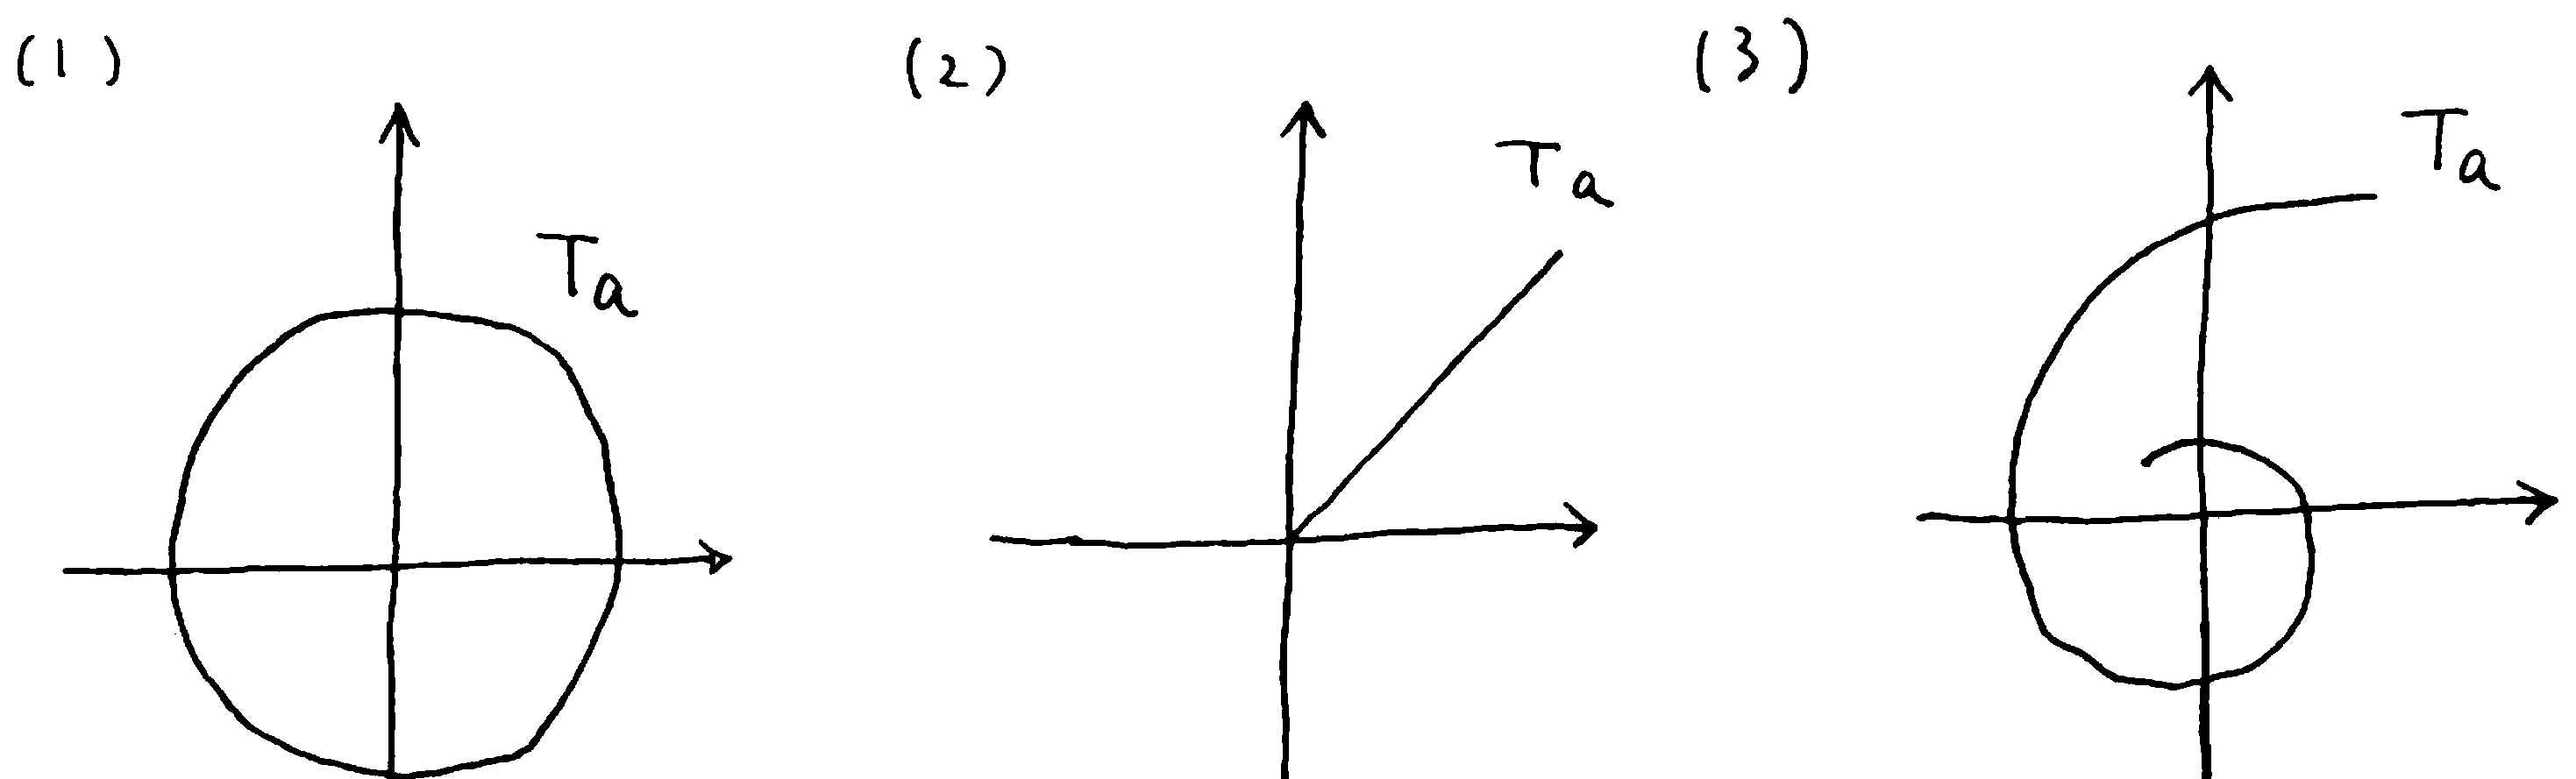
\includegraphics[width=0.75\linewidth]{fig_p27_a.png}
\end{center}

其次看$(\omega)_0$处的样子。设$\operatorname{ord}(\omega)=m>0$，则
$\omega=(a_mz^m+a_{m+1}z^{m+1}+\cdots)dz^{\otimes2}$，$a_m\neq0$。
故取满足$g(z)^2=a_mz^m+a_{m+1}z^{m+1}+\cdots$的$g(z)$，便有
$g(z)=b_{m/2}z^{m/2}+b_{m/2+1}z^{m/2+1}+\cdots$。

（1）$m$为偶数的情形。令$m=2m'$，则
$\psi(z)=\int g(z)dz=\frac{1}{m'+1}b_{m'}z^{m'+1}+\cdots$，
故$T_0$同胚于在原点相交的$m+2$条半直线。

% ===== 原书 p.22 =====
$T_a$如下图所示。

\begin{center}
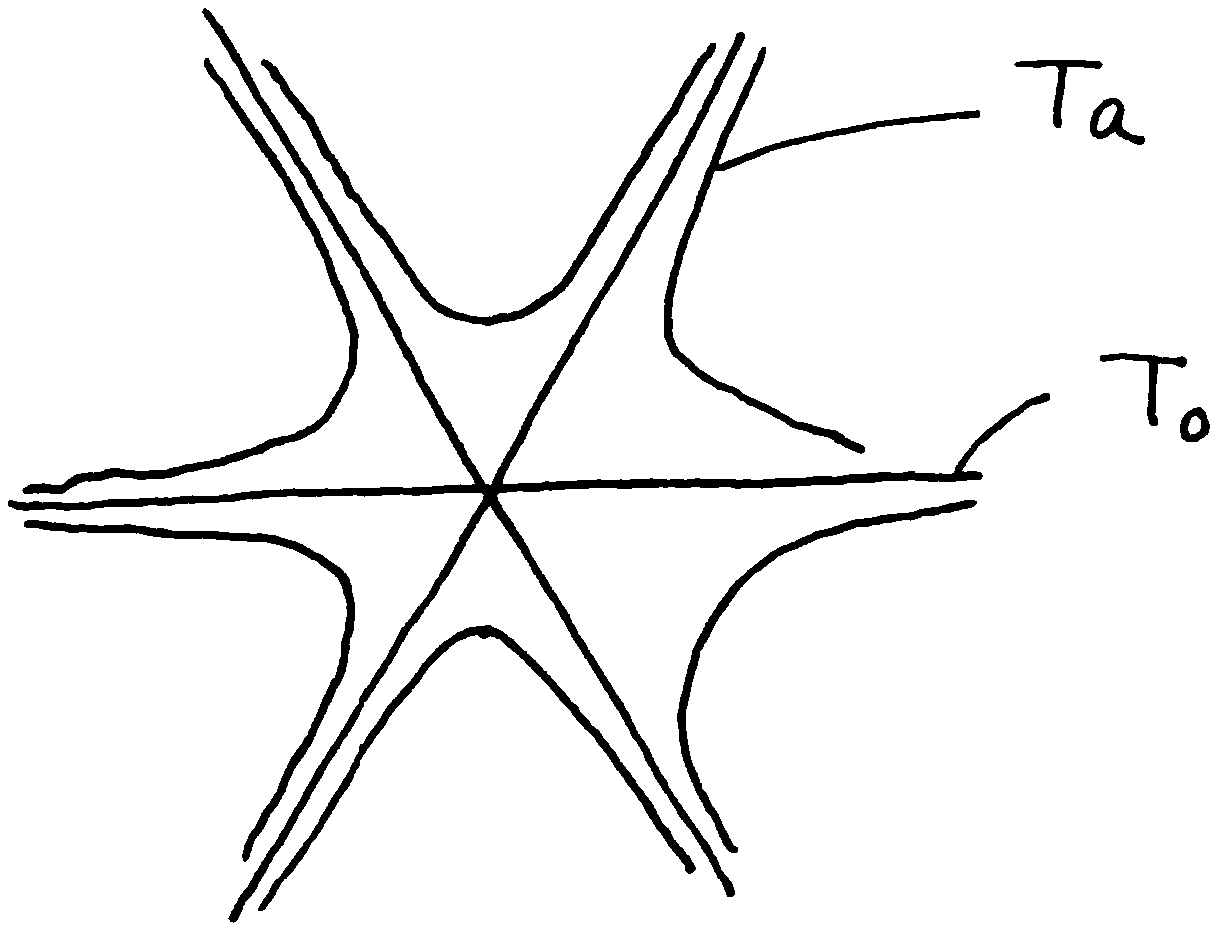
\includegraphics[width=0.42\linewidth]{fig_p28_a.png}
\end{center}

（2）$m$为奇数的情形。令$z^{1/2}=u$，在由$u$决定的分歧覆盖上，$\psi(z)$为
\[
\psi(z)=\frac{2}{m+2}b_{m/2}u^{m+2}+\cdots
\]
把它放回$z$平面上考虑，$T_0$仍同胚于在原点相交的$m+2$条半直线。
$T_a\cup T_{-a}$如下图所示。（此处须注意，$T_a\cup T_{-a}$不依赖于$u$的分支取法。）

\begin{center}
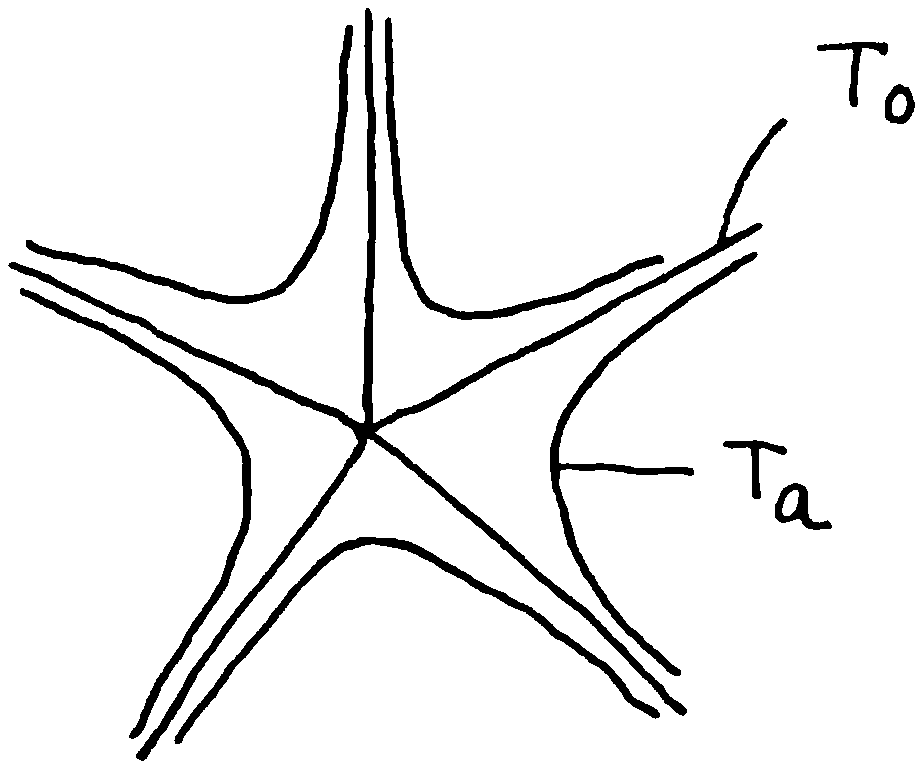
\includegraphics[width=0.38\linewidth]{fig_p28_b.png}
\end{center}

下面据此看$X$整体给出怎样的叶状结构。例如$X$的亏格为$1$，$p$为$X$上一点。
考察仅在$p$处有极点、在$q_0$与$q_1$处有单零点的二次微分$\omega$，
并且$p$处的展开系数为$b_{-1}\in\R$即$a_{-2}\in\R_{>0}$的情形。
此时出现下图那样的叶状结构。（这是切开的图。）

\begin{center}
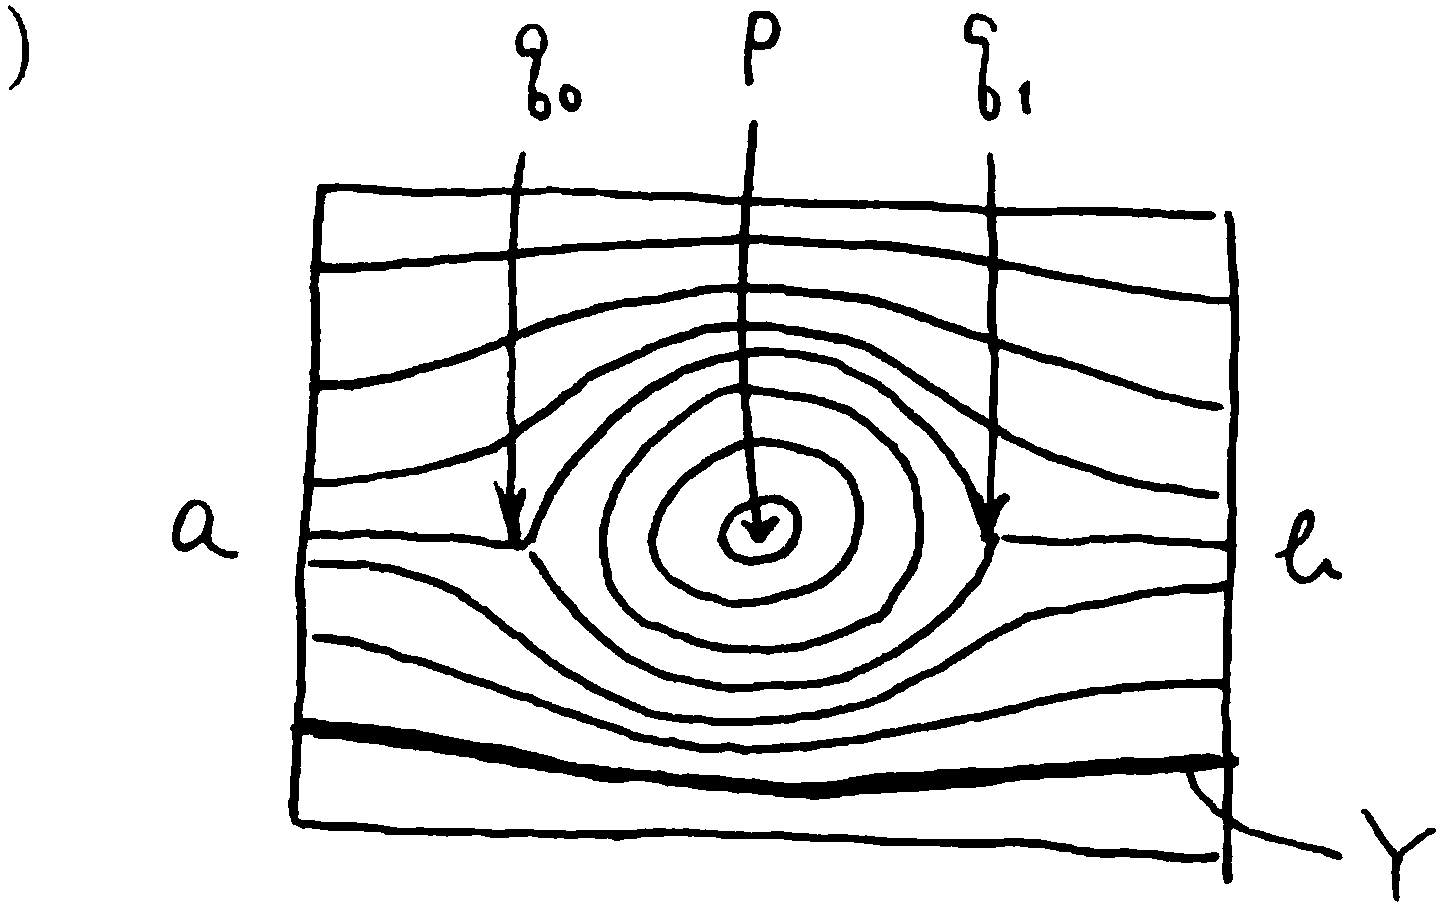
\includegraphics[width=0.55\linewidth]{fig_p28_c.png}
\end{center}

% ===== 原书 p.23 =====
此时，「$\omega$有单零点」这一条件在$H^0(X,(\Omega^1_X(D))^{\otimes2})$中是开条件，
而$a_{-1}\in\R_{>0}$是实余维$1$的条件。以$\R_{>0}$作乘法换掉$\omega$，叶状结构本身并不改变，
故上图以实$2$维自由度出现。须注意，图中$a$与$b$一致，$Y$附近的叶状结构同构于$S^1$，
这两件事等价。要使$a$与$b$一致，还须再加一个余维$1$的条件。
在该条件下把$\omega$取来换去，连结$q_0$与$q_1$的曲线绕$p$一周所得区域的面积随之改变。（下图）

\begin{center}
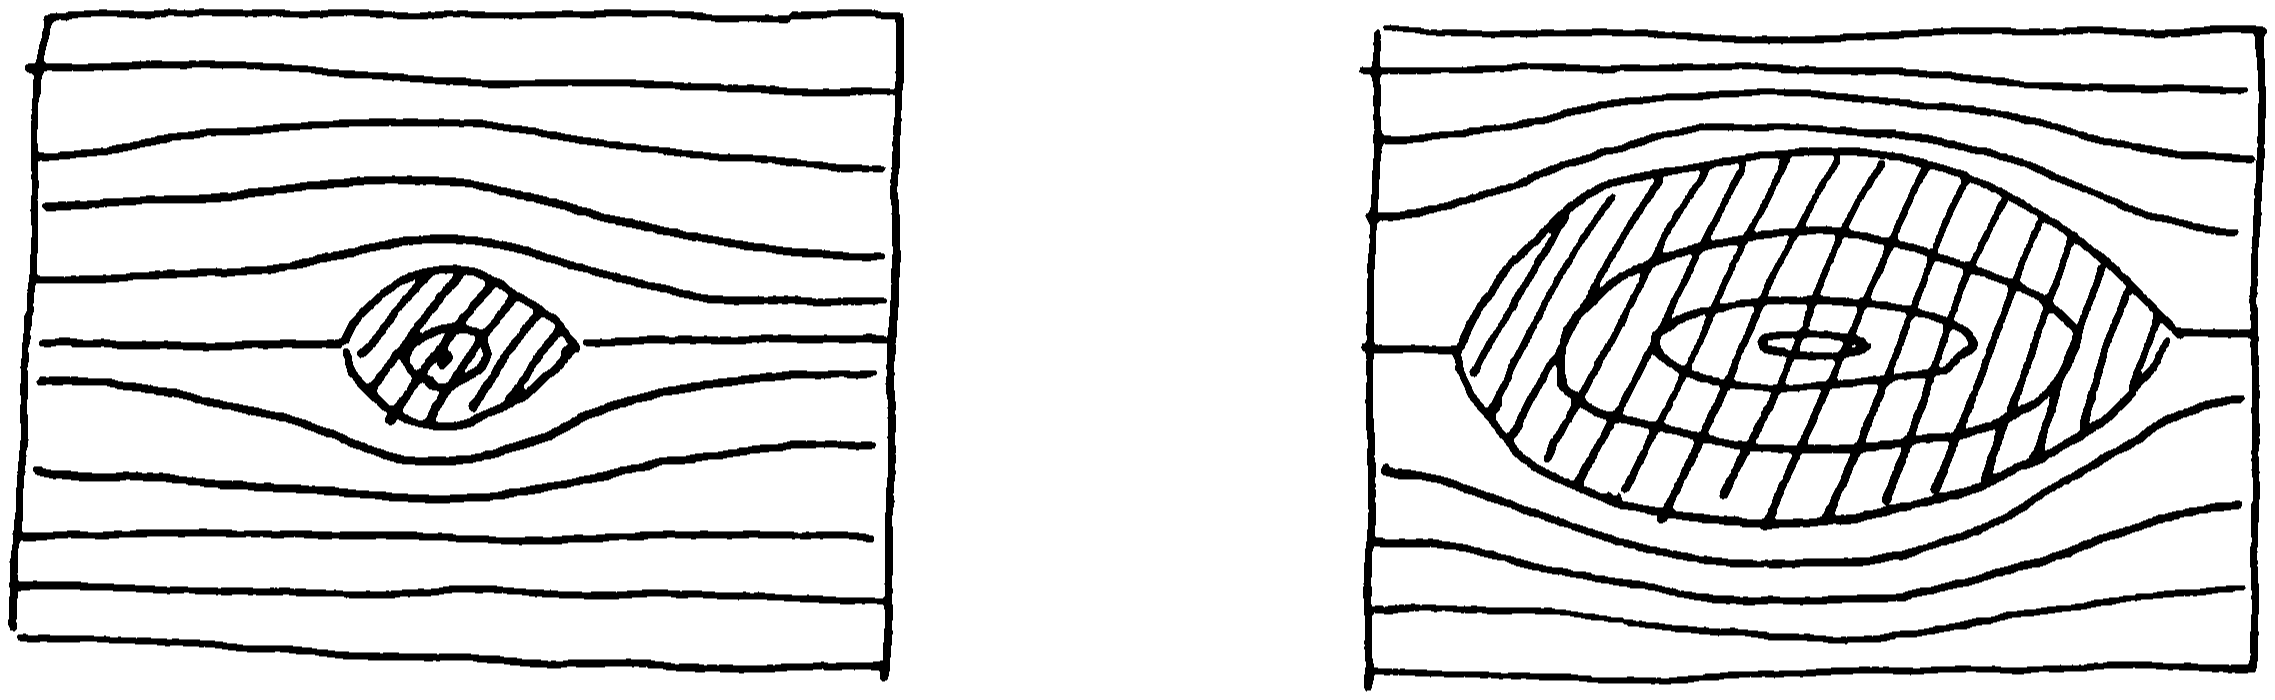
\includegraphics[width=0.6\linewidth]{fig_p29_a.png}
\end{center}

取有一维参数的参数族，使面积不断增大，则应落到
$H^1(X,(\Omega^1_X(D))^{\otimes2})-\{0\}/\R^+\cong S^3$中某点。
若一切顺利，可以预测只能取到唯一一个这样的二次微分：图中斜线部分占去几乎所有的点。
后文可知这是正确的。此时成下图。粘合的状况一般如上图那样。

\begin{center}
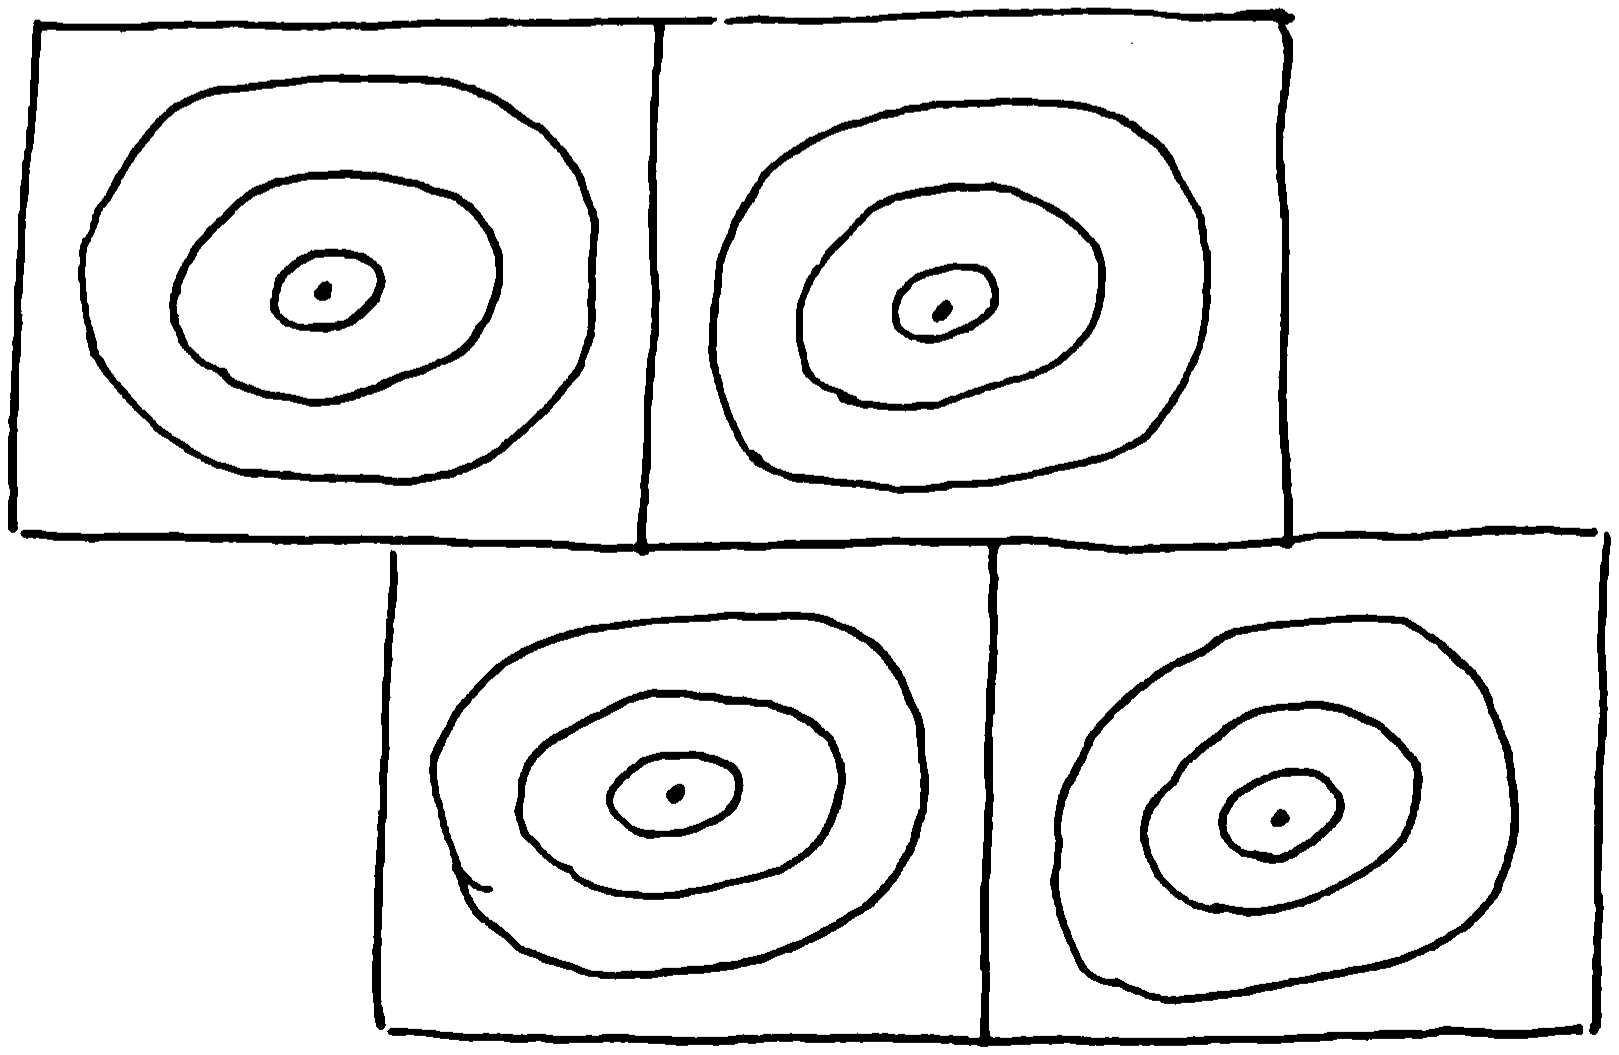
\includegraphics[width=0.6\linewidth]{fig_p29_b.png}
\end{center}

% ===== 原书 p.24 =====
进而，把与$p$周围小闭曲线同伦的、同胚于$S^1$的轨道全部除去，则得下图那样的$1$-骨架。

\begin{center}
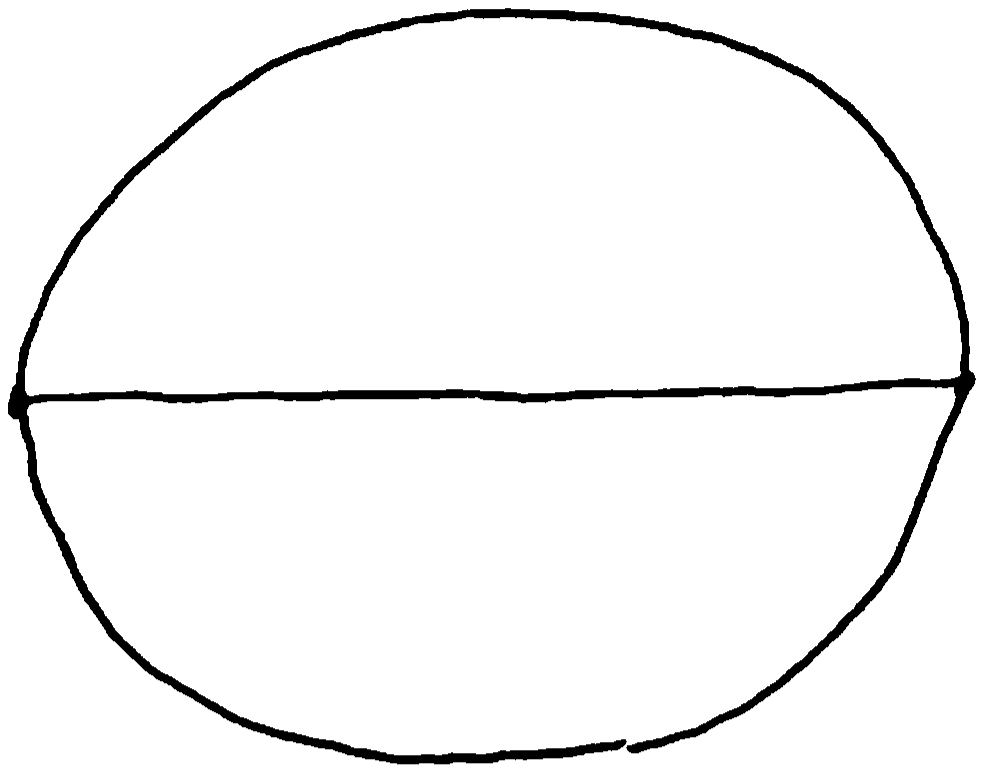
\includegraphics[width=0.3\linewidth]{fig_p30_a.png}
\end{center}

这样给出椭圆曲线与$1$点后，以$\R_{>0}$为模，上图那样的图型只有$1$种。
（实际上依椭圆曲线不同，也出现下图那样的情形。）

\begin{center}
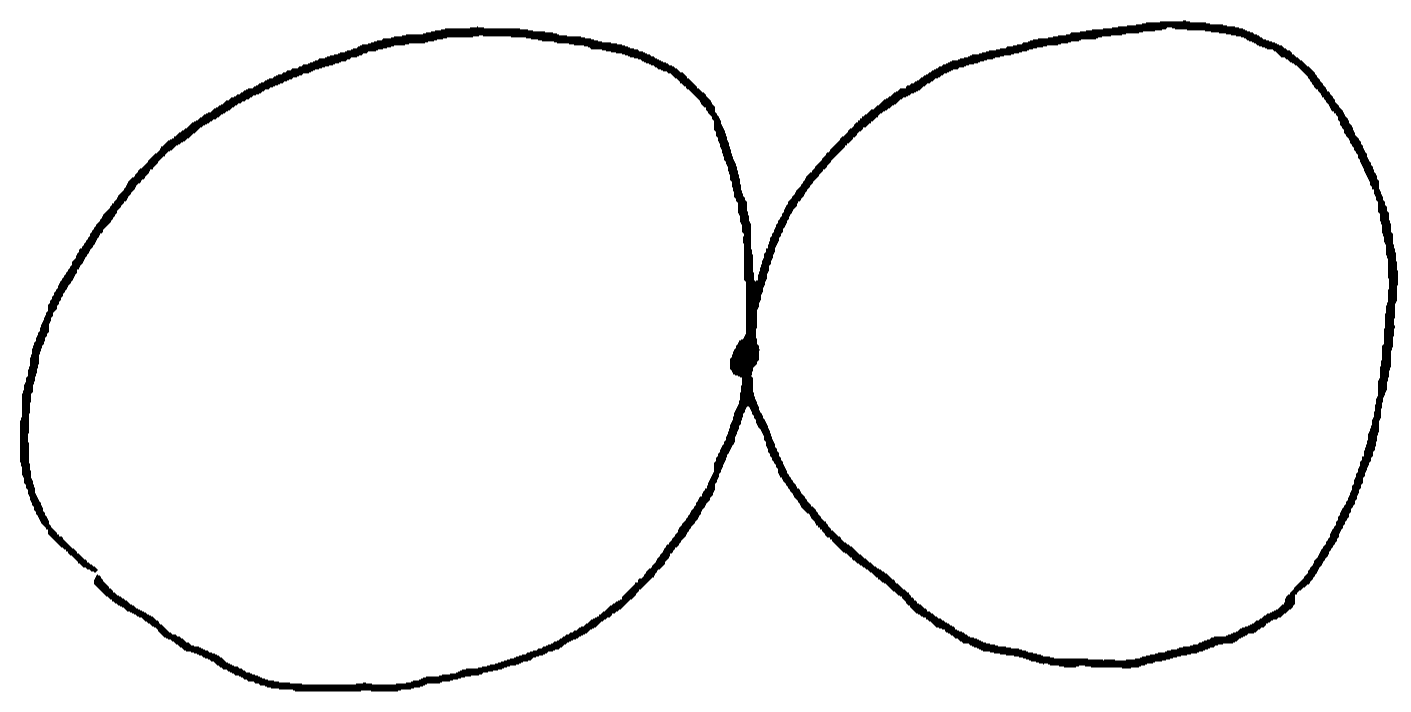
\includegraphics[width=0.34\linewidth]{fig_p30_b.png}
\end{center}

证明这种二次微分的存在与唯一性，是本章的目的。

% Theorem 2.1（原书印 Theorem 2.1）
\begin{theorem}
设$X$为紧 Riemann 面，$p_1,\dots,p_n$为$X$上相异的$n$点，$r_1,\dots,r_n$为$\R_{>0}$的元。
此时存在唯一的二次微分，具有下列性质。
\begin{enumerate}[label=(\arabic*),leftmargin=2.6em,itemsep=2pt,topsep=4pt]
\item 在$p_i$周围，$\omega$有下列展开
\[
\omega=\left(r_iz_i^{-2}+O\left(\frac{1}{z}\right)\right)dz^{\otimes2}
\]
\item 取$\gamma_i$为$p_i$周围的小闭曲线，则
\[
X^{(1)}=X-\bigcup_{i=1}^n\{\delta\mid\delta\text{是与}S^1\text{同胚的轨道，且与}\gamma_i\text{同伦}\}
\]
是$X$的测度$0$集。
\end{enumerate}
\end{theorem}

% ===== 原书 p.25 =====
此外，此时$X^{(1)}$为$1$维 CW 复形。

证明将在§2.3、§2.4给出。

% Definition 2.1（原书印 Definition 2.1）
\begin{definition}
具有定理 2.1 的(2)的性质的二次微分，称为具闭轨道的二次微分。
\end{definition}

% §2.2（原书印「§2.2 QUADRATIC DIFFERENTIAL FORM と RIBBON GRAPH」）
\subsection{二次微分形式与带状图}

现给定 Riemann 面$X$及其上$n$点$p_1,\dots,p_n$以及$r_1,\dots,r_n\in\R_+=\{r\in\R\mid r>0\}$时，
考虑满足定理 2.1 条件的二次微分$\omega$。
在$X^0-\{p_1,\dots,p_n\}-(\omega)_0$上，如前所述由$\omega$决定平坦度量，
由此在$X^{(1)}$上诱导度量。又$X^{(1)}$位于$X$上，故在下列意义下成为带状图（ribbon graph）。

% Definition 2.2（原书印 Definition 2.2 (ribbon graph)）
\begin{definition}[带状图]
无边界的一维 CW 复体$K$（即对任意顶点，以它为端点的棱至少有$2$条）具有带状结构（ribbon
structure）$R$，指的是对每个顶点$v$，在$E_v=\{e:\text{棱}\mid v\text{是}e\text{的端点}\}$上
定好循环次序。用图表示循环次序时，使用下图中任一个。
\end{definition}

\begin{center}
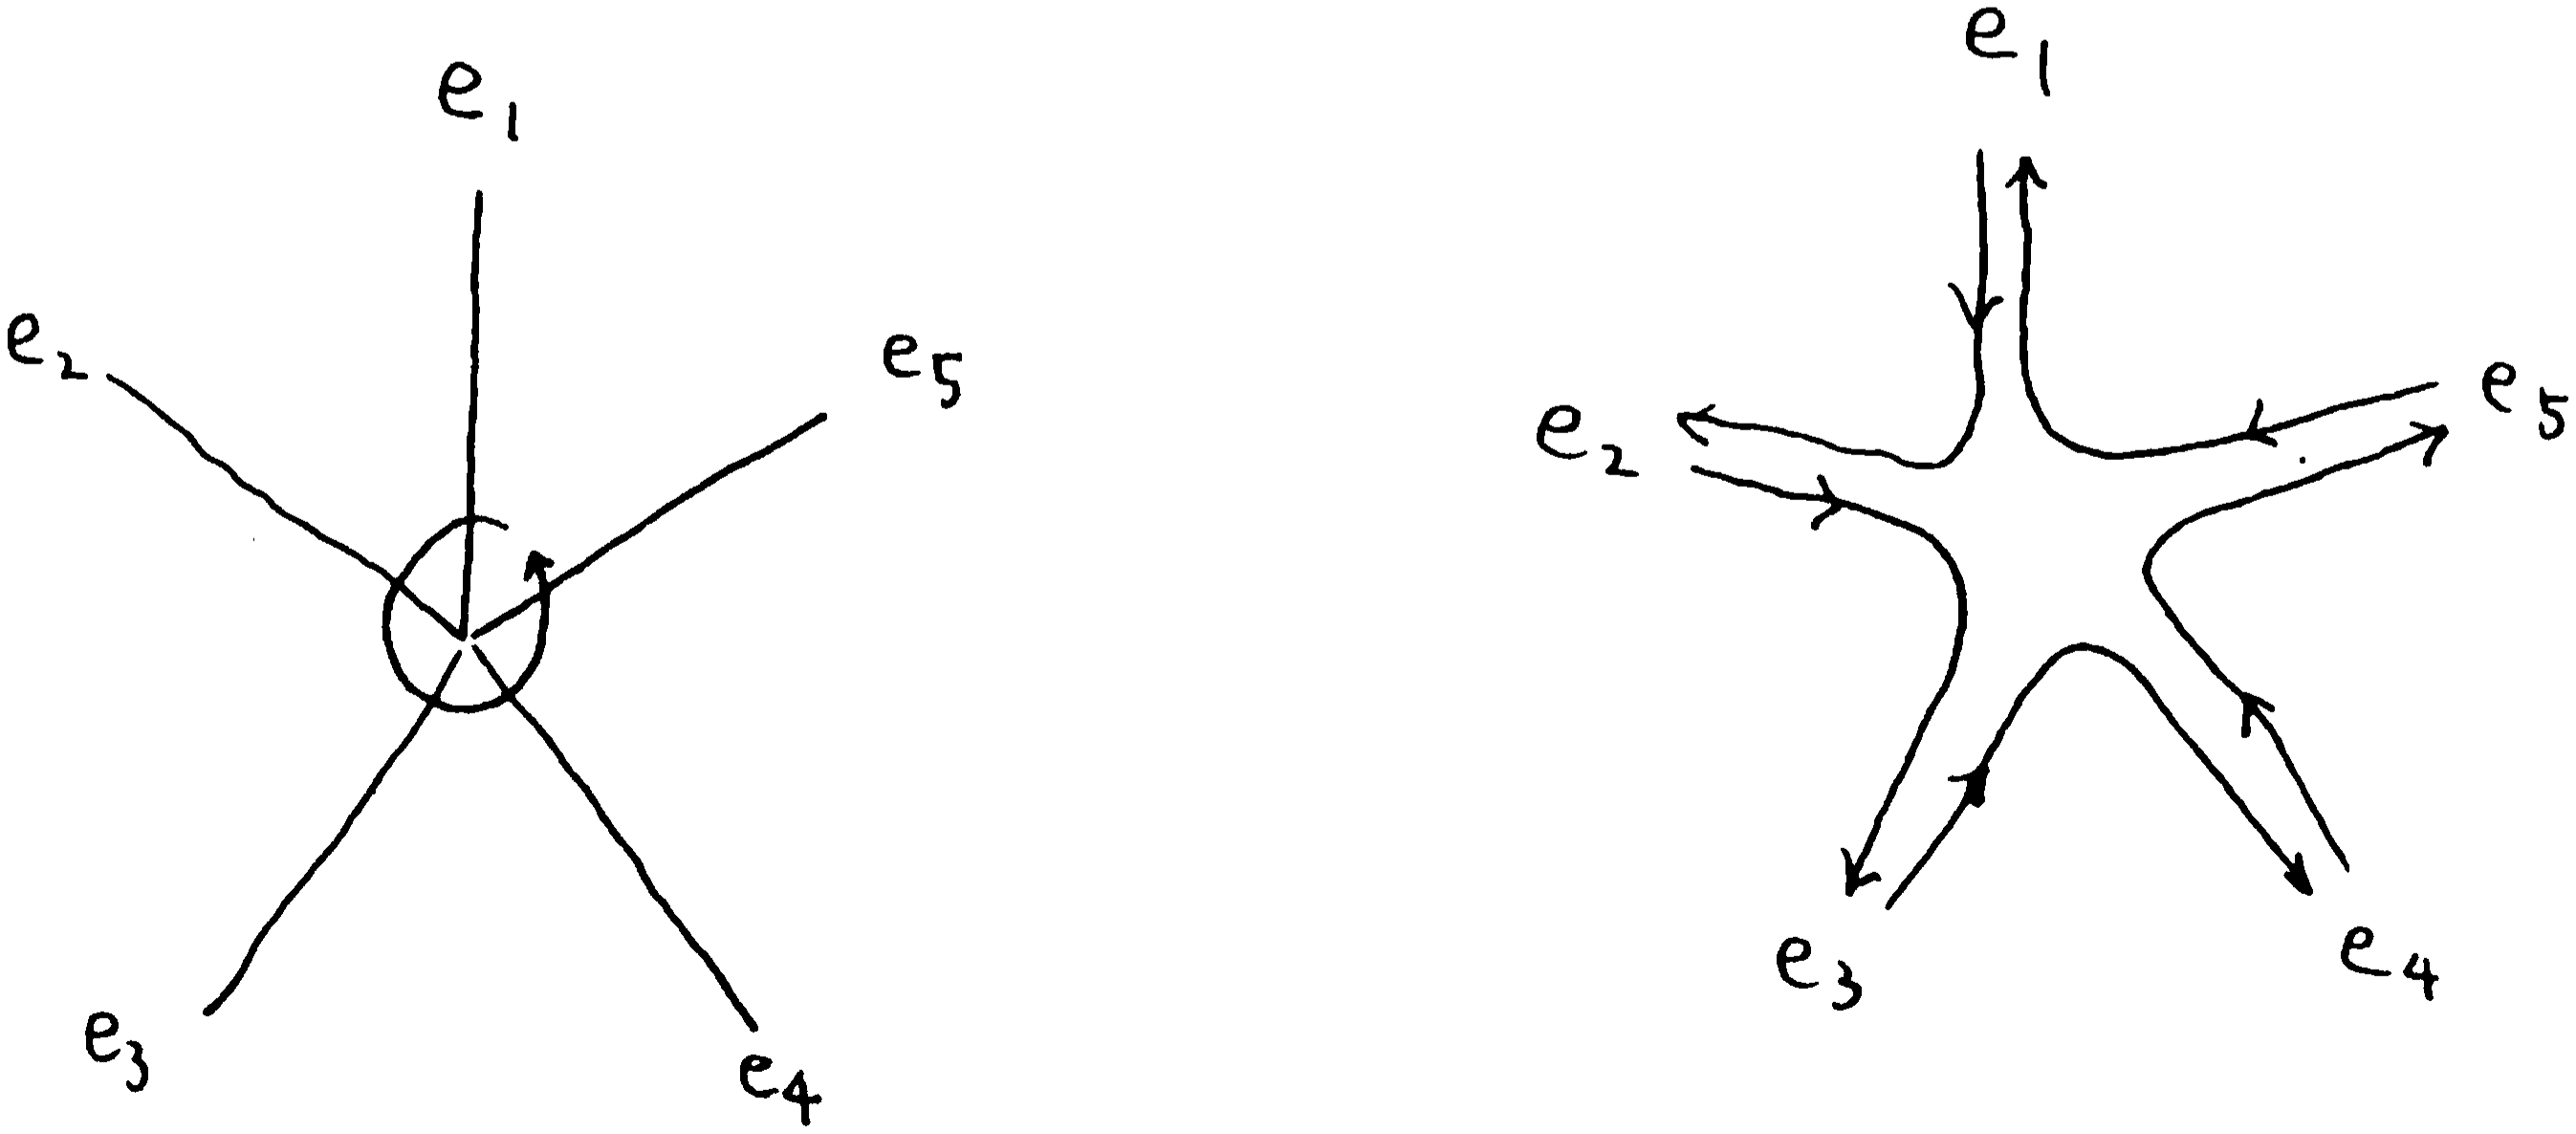
\includegraphics[width=0.72\linewidth]{fig_p31_a.png}
\end{center}

% Example（原书印 Example.，未编号；按原书排成不编号的黑体提示语，不占 example 计数器）
\noindent\textbf{例.}
设$K$为由顶点集$V(K)=\{v_1,v_2\}$、棱集$E(K)=\{e_1,e_2,e_3\}$给出，
且$e_i$（$i=1,2,3$）的端点集表为$\operatorname{end}(e_i)=\{v_1,v_2\}$的图。

% ===== 原书 p.26 =====
\begin{center}
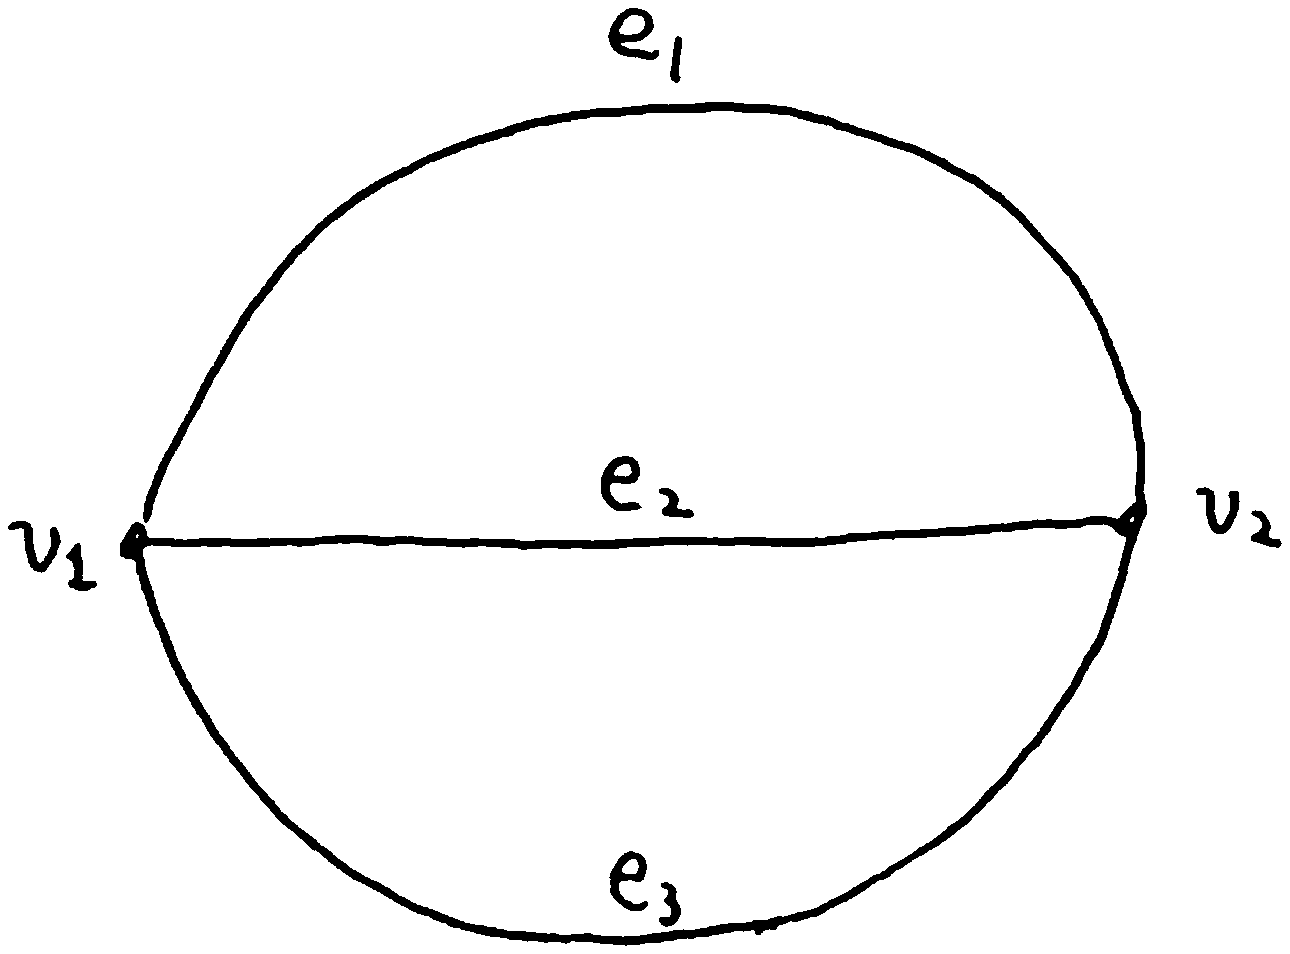
\includegraphics[width=0.32\linewidth]{fig_p32_a.png}
\end{center}

$E(v_1)=\{e:\text{棱}\mid v_1\text{是}e\text{的端点}\}$的循环次序给定为$e_3\to e_2\to e_1$，
$E(v_2)$的循环次序给定为$e_3\to e_2\to e_1$时，其带状图如下表示。

\begin{center}
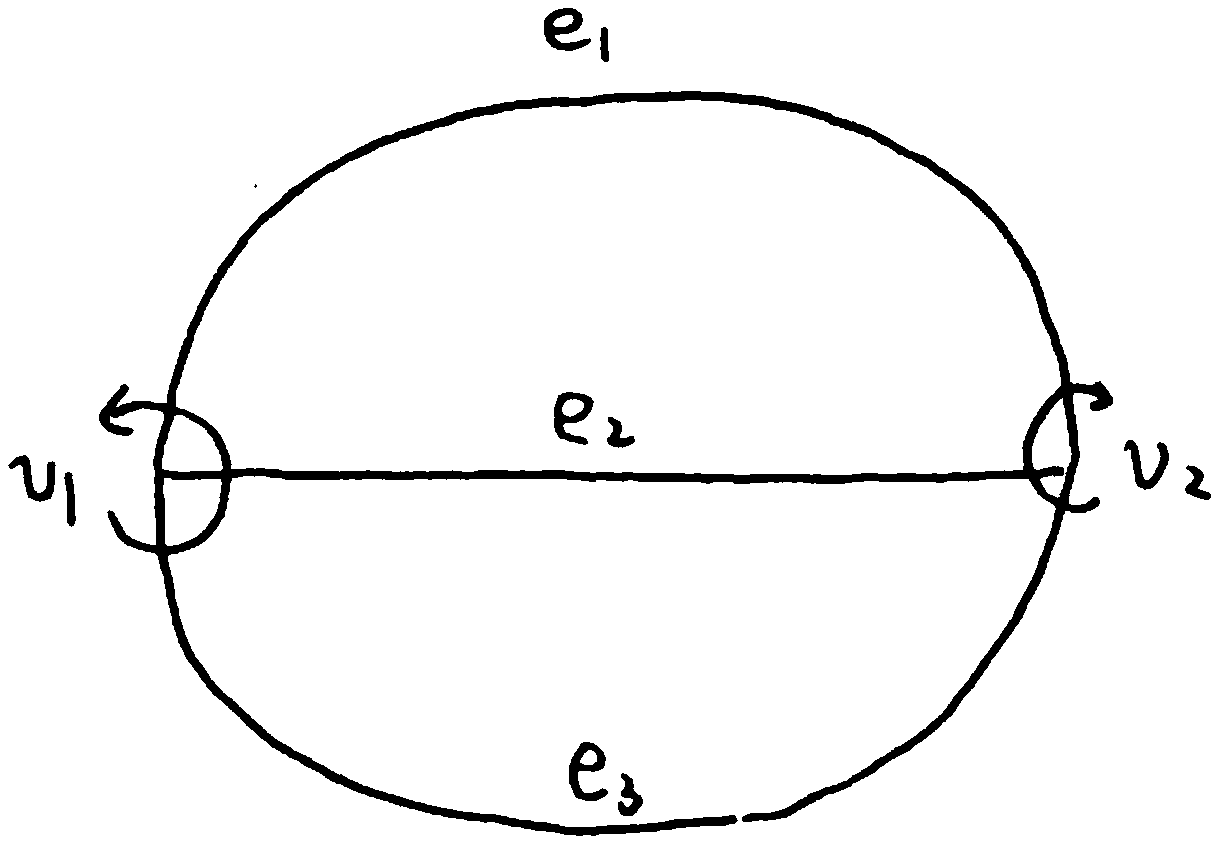
\includegraphics[width=0.40\linewidth]{fig_p32_b1.png}\hspace{1.5em}或\hspace{1.5em}%
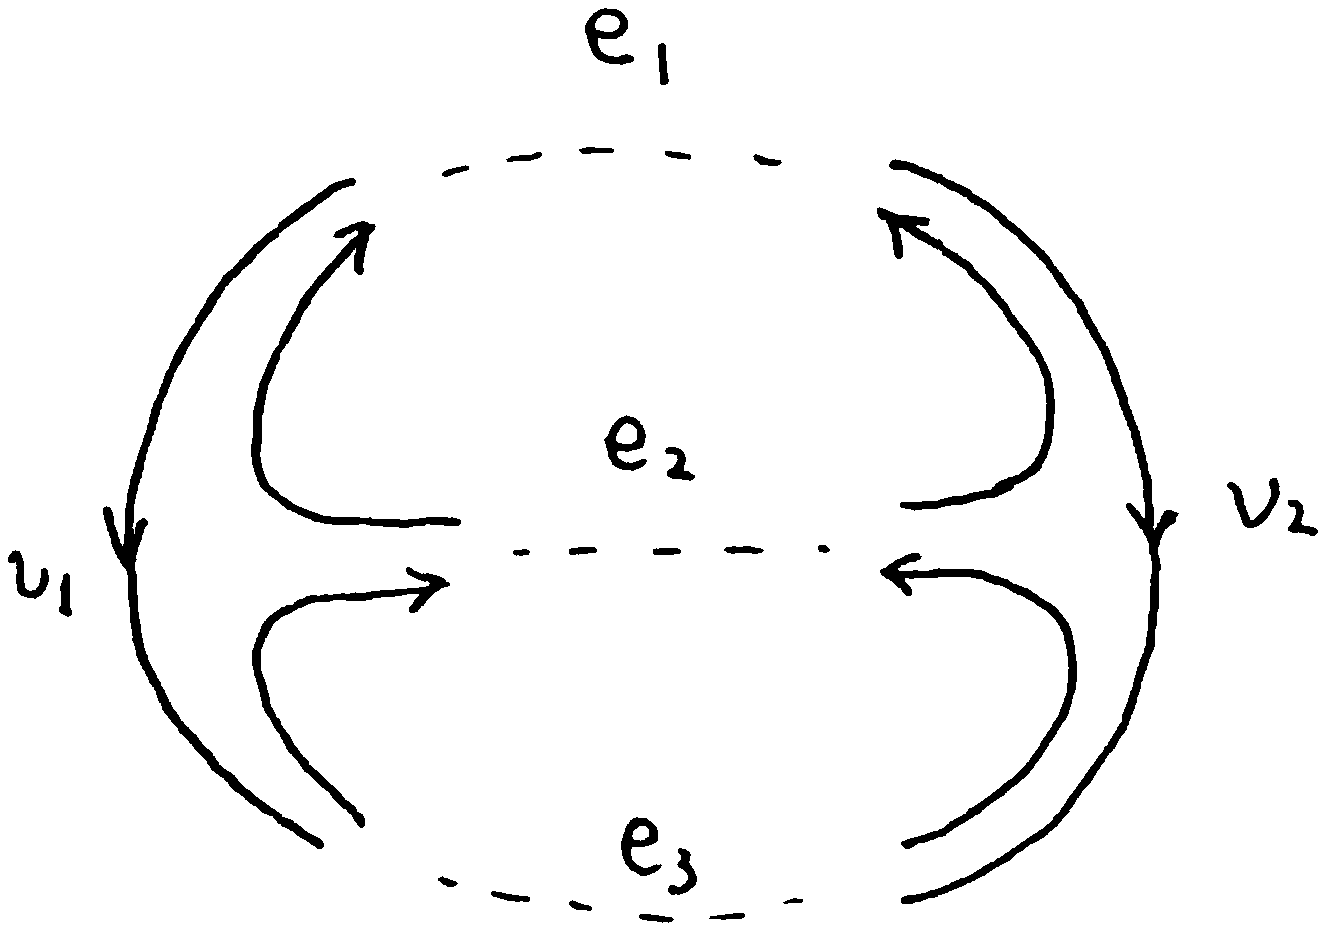
\includegraphics[width=0.40\linewidth]{fig_p32_b2.png}
\end{center}

后一情形也有把两侧带方向的带状长条插入棱中、使整体箭头相连来表示的做法。（下图）

\begin{center}
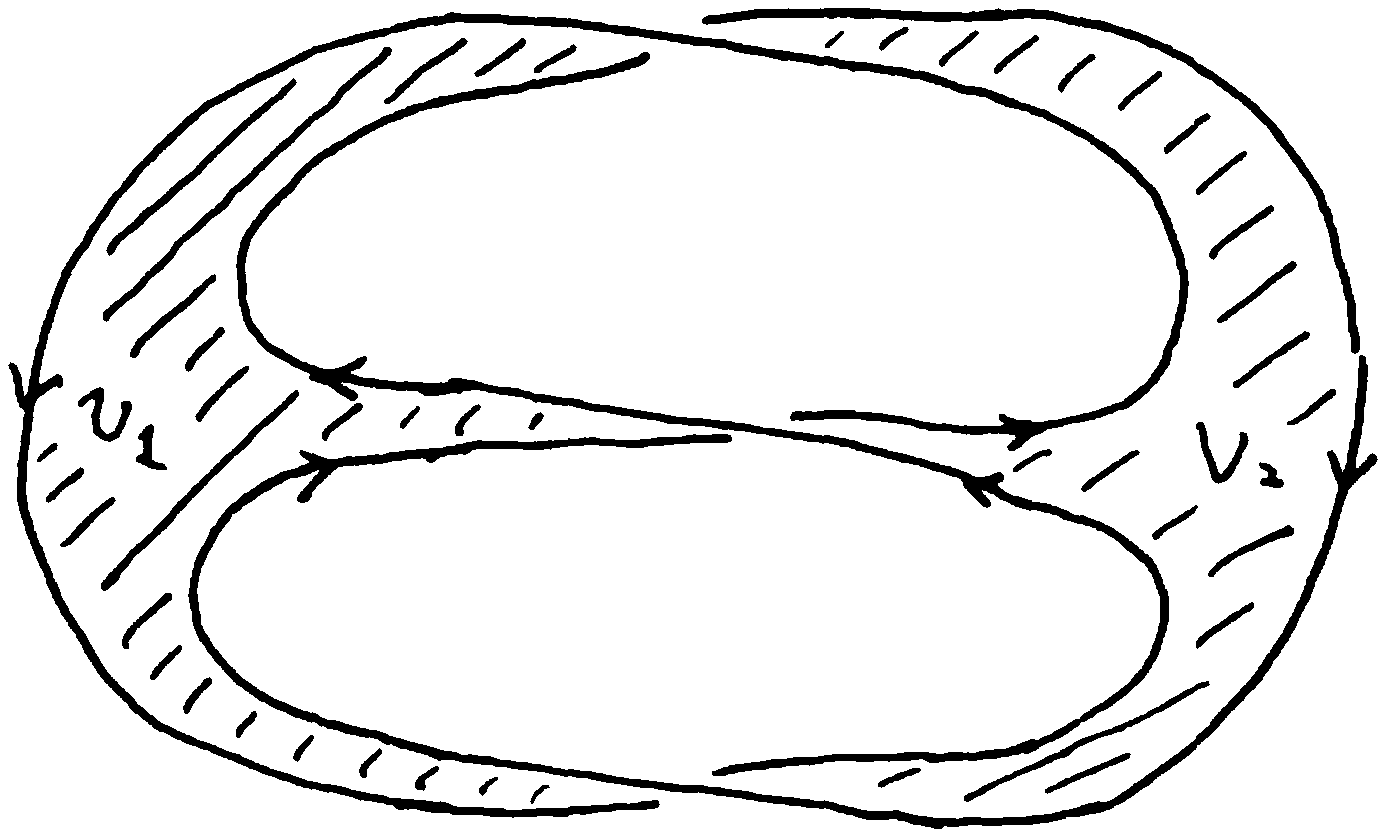
\includegraphics[width=0.45\linewidth]{fig_p32_c.png}
\end{center}

% Definition 2.3（原书印 Definition 2.3 (metrized ribbon graph)）
\begin{definition}[带度量带状图]
带状图$(K,R)$上的度量结构（metric structure），指给带状图的每条棱赋正数$l_i$作为「长度」。
\end{definition}

这样，由 Riemann 面、其上$n$点以及正数$r_1,\dots,r_n$的组
$(X,p_1,\dots,p_n,r_1,\dots,r_n)$这样的数据，构成带度量带状图$(K,R,M)$，而$X$的

% ===== 原书 p.27 =====
亏格$g=g(X)$及点的个数$n$，可从$(K,R,M)$如下读出。
首先，把带状图如图 1 那样表示时，边界的个数即给出$n$。
进而，$K$作为拓扑空间的 Euler 数$=\#V(K)-\#E(K)$等于$2-2g-n$，由此可读出$g$。即
\[
g=\frac{1}{2}(2-n+\#E(K)-\#V(K)).
\]
称$(g,n)$为带状图的型。即使图相同，带状结构的给法不同，其型$(g,n)$也会改变。
例如下图(1)为$(g,n)=(1,1)$，(2)为$(g,n)=(0,3)$。

\begin{center}
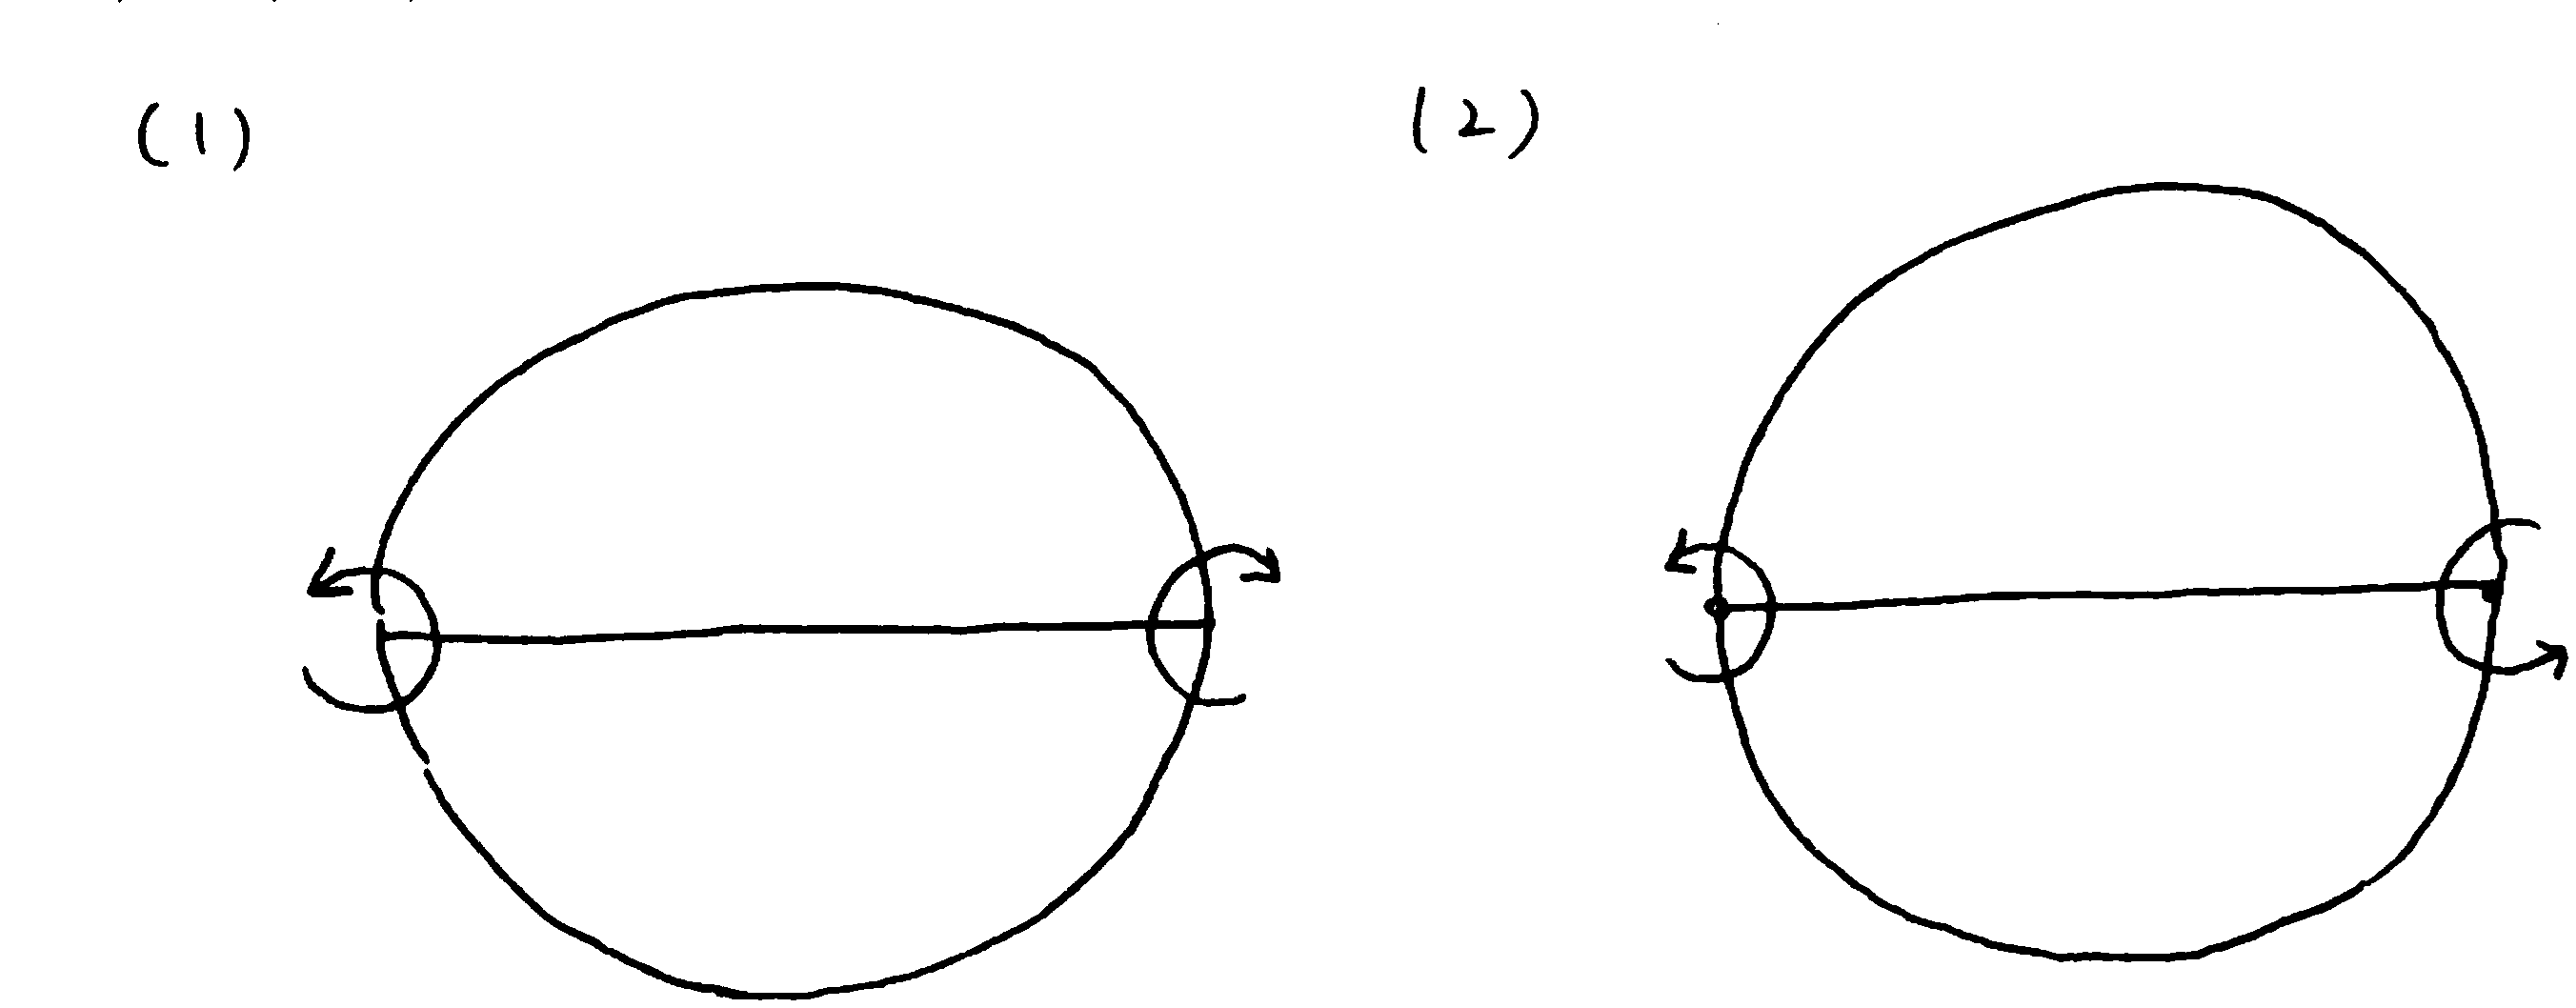
\includegraphics[width=0.6\linewidth]{fig_p33_a.png}
\end{center}

最后，给定带度量带状图$(K,R,M)$时，构造 Riemann 面$X$、其上点$p_1,\dots,p_n$以及在
$p_1,\dots,p_n$处有二阶极点的二次微分$\omega$，使由此得到的带度量带状图为$(K,R,M)$，
以此结束本节。设带状图的边界分支数为$n$，$\partial_1,\dots,\partial_n$为边界，
依次取参与$\partial_i$的棱为$e_{i,1},\dots,e_{i,k_i}$。（这除循环置换外确定。）
记$e_{i,j}$的长度为$s_{i,j}$，令$s_i=\sum_{j=1}^{k_i}s_{i,j}$。
现准备$n$个去心圆盘$D_i^*$，令
\[
D_i^*=\{z_i\in\C\mid0<|z_i|<1\}\subset\overline{D}_i^*=\{z_i\in\C\mid0<|z_i|\le1\}.
\]
把$\overline{D}_i^*$沿其边界$\{z_i\mid|z_i|=1\}$如下粘合。
现设对$(i,j)\neq(i',j')$，有$e_{i,j}=e_{i',j'}$。（下图）

\begin{center}
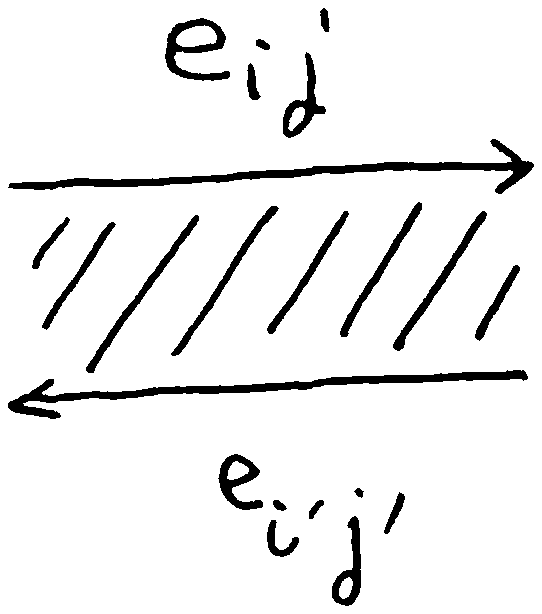
\includegraphics[width=0.24\linewidth]{fig_p33_b.png}
\end{center}
